% =============================================================================
% Draft v2 -- UET vs RoCE/DCQCN in htsim, full-bisection fabrics only.
% Numbers: fidelityRuns/results (flat 1os + rail, 5 seeds) and
%          ablationMultipath/results (16 MB, 5 seeds).
% Figures: bin/make_paper_figs.py (fig_*.png, regenerated from the CSVs);
%          f08/f09/f10 copied unchanged from fidelityRuns/graphs.
% Topology / mechanism / workload illustrations are TikZ, inline below.
% Build:  pdflatex main && bibtex main && pdflatex main && pdflatex main
% =============================================================================
\documentclass[conference]{IEEEtran}
\IEEEoverridecommandlockouts
\usepackage{cite}
\usepackage{amsmath}
\usepackage{graphicx}
\usepackage{booktabs}
\usepackage{multirow}
\usepackage{array}
\usepackage{url}
\usepackage{xcolor}
\usepackage{tikz}
\usepackage{placeins}
\usepackage{balance}
\usetikzlibrary{arrows.meta,calc,decorations.pathreplacing}
\definecolor{fabric}{HTML}{2F6DA8}
\definecolor{nvl}{HTML}{B4671F}
\definecolor{roce}{HTML}{0072B2}
\definecolor{uet}{HTML}{D55E00}
\definecolor{flowA}{HTML}{0072B2}
\definecolor{flowB}{HTML}{CC79A7}
\graphicspath{{figs/}}
\renewcommand{\topfraction}{0.9}
\renewcommand{\dbltopfraction}{0.85}
\renewcommand{\textfraction}{0.07}
\renewcommand{\floatpagefraction}{0.8}
\renewcommand{\dblfloatpagefraction}{0.8}
\setcounter{dbltopnumber}{2}

\newcommand{\roce}{RoCE/DCQCN}
\newcommand{\uet}{UET}
\newcommand{\todo}[1]{\textcolor{red}{[TODO: #1]}}
\newcommand{\wl}[1]{\textsf{#1}}
% eight nodes on a circle, named <prefix>0..<prefix>7 (workload figure)
\newcommand{\ring}[1]{%
  \foreach \i in {0,...,7} \node[nd] (#1\i) at ({90-\i*45}:0.78) {\i};}

\begin{document}

\title{Spray or Pause? A Controlled Simulation Study of\\
Ultra Ethernet Transport and RoCE/DCQCN for AI Cluster Fabrics}

\author{\IEEEauthorblockA{Technion -- Israel Institute of Technology}}

\maketitle

% -----------------------------------------------------------------------------
\begin{abstract}
AI clusters are increasingly limited by their network, and two designs compete
for the back-end fabric. RoCE with PFC and DCQCN keeps the fabric
\emph{lossless} and pins each flow to one path. The Ultra Ethernet Transport
(UET) lets the fabric \emph{drop}: it sprays packets across all paths, trims
on overflow and retransmits quickly. We compare the two in the htsim
packet-level simulator with identical full-bisection topologies, link speeds
and traffic, on 400\,Gb/s fat-trees and on rail-optimized GPU clusters with
NVLink. UET is faster in 28 of 34 fat-tree configurations, by a median
6.4$\times$ on permutation traffic; RoCE/DCQCN wins only when a single
receiver port is the bottleneck. A multipath ablation, which restricts UET to
one path and splits RoCE flows over up to eight queue pairs, separates the
two effects: per-packet spraying explains about 70\% of UET's advantage on
permutation traffic and none of it on incast, and with both stacks on a
single path UET's transport is still 1.3--1.8$\times$ faster. On
rail-optimized GPU clusters with NVLink, rail placement speeds up RoCE/DCQCN by
8--41\% and UET by 3--10\% compared with a flat placement, and brings
RoCE/DCQCN within 1.02--1.33$\times$ of UET on MoE all-to-all, while UET keeps
a 1.7--4.6$\times$ lead on all-reduce.
\end{abstract}

\begin{IEEEkeywords}
Ultra Ethernet, RoCE, DCQCN, PFC, packet spraying, multipath, rail-optimized,
NVLink, AI training, collective communication, htsim
\end{IEEEkeywords}

% -----------------------------------------------------------------------------
\section{Introduction}

Distributed training and inference are dominated by collective communication:
all-reduce for gradient synchronization, all-to-all for Mixture-of-Experts (MoE)
routing, and many-to-one gathers. These patterns are bursty and synchronized,
and they create exactly the congestion that commodity datacenter transports
handle worst. The back-end fabric therefore matters for end-to-end job time.

Two philosophies compete for that fabric. The incumbent, RDMA over Converged
Ethernet (RoCEv2), relies on Priority Flow Control (PFC)~\cite{pfc} to make the
network lossless. DCQCN~\cite{dcqcn} slows senders before buffers fill. Because
RoCE expects near-in-order delivery, each flow is pinned to a single ECMP path.
The Ultra Ethernet Consortium's transport (UET)~\cite{uec-spec,uec-design}
takes the opposite approach. It tolerates loss instead of preventing it. Every
packet is sprayed across all paths, switches \emph{trim} rather than drop
overflowing packets~\cite{ndp} so that the receiver can request a fast
retransmission, and a sender-based congestion controller (NSCC) reacts to delay
and ECN.

Which approach is better, on which traffic, and why? Vendor results are hard to
compare because they change the transport, the topology and the hardware all
at once. Moreover, UET bundles two separate ideas, per-packet multipath and a
loss-tolerant transport, and an end-to-end comparison cannot tell which one
matters. We implement both stacks in one packet-level simulator,
htsim~\cite{ndp}, change only the transport, and then take the multipath
dimension apart. Our contributions:

\begin{itemize}
  \item \textbf{A controlled comparison} of UET and RoCE/DCQCN on 400\,Gb/s
        full-bisection fat-trees of 128 and 1024 nodes across seven traffic
        patterns, each repeated with five ECMP seeds and tested for
        significance (\S\ref{sec:flat}).
  \item \textbf{An accounting of what each stack pays}: retransmitted bandwidth
        for UET, PFC pause time and idle links for RoCE/DCQCN (\S\ref{sec:cost}).
  \item \textbf{Rail-optimized GPU clusters with NVLink} of 1024 and 2048
        GPUs, with NVLink modelled as a second, intra-server topology
        (\S\ref{sec:rail}). Rail placement helps \emph{both} transports, and
        on MoE all-to-all it brings RoCE/DCQCN close to UET.
  \item \textbf{A multipath ablation} that runs UET on a single path and
        splits each RoCE flow over $K\in\{1,2,4,8\}$ queue pairs, separating
        the contribution of spraying from that of the transport
        (\S\ref{sec:ablation}).
\end{itemize}

% -----------------------------------------------------------------------------
\section{Background}

\textbf{RoCE, PFC and DCQCN.}
RoCEv2 carries RDMA over UDP/IP. PFC makes a priority class lossless: when an
ingress buffer crosses a threshold, the switch pauses its upstream neighbour.
This avoids loss but can spread congestion to flows that do not use the hot
link (head-of-line blocking, congestion trees)~\cite{rdma-scale}. DCQCN adds
end-to-end rate control. Switches ECN-mark packets above a queue threshold, the
receiver returns congestion notification packets (CNPs), and the sender cuts its
rate multiplicatively, then recovers through timer- and byte-counter-driven
increase stages~\cite{dcqcn}. Each flow, or more precisely each queue pair
(QP), follows one ECMP path, so long flows that hash onto the same link collide
for their whole lifetime~\cite{hedera}. Libraries such as NCCL therefore often
open several QPs per connection to obtain some path diversity.

\textbf{Ultra Ethernet Transport.}
UET~\cite{uec-spec,uec-design} targets the same RDMA semantics on a best-effort
Ethernet fabric. Its key mechanisms are:
(i) \emph{per-packet spraying} across many paths, selected by an entropy value
in the header~\cite{spray,reps};
(ii) \emph{packet trimming}: an overflowing switch forwards only the header,
which triggers a NACK and a fast retransmit instead of a timeout~\cite{ndp};
(iii) an out-of-order-tolerant receiver; and
(iv) NSCC, a sender-based window controller driven by delay and
ECN~\cite{reps}. UET is a recent standard, and there are still few independent
evaluations of it against the RoCE baseline it aims to replace.

% -----------------------------------------------------------------------------
\section{Methodology}
\label{sec:method}

\subsection{Simulator and stacks}
We use htsim~\cite{ndp}, which includes models of both the UEC transport and
RoCE. Table~\ref{tab:stacks} lists the two configurations. Everything except
the transport is shared: topology files, link speeds, link latencies and
traffic matrices. MTU is each stack's native default (4000\,B for RoCE, 4150\,B
for UET), a difference of a few percent in per-packet overhead. UET runs with
sender-based congestion control only, without its optional receiver-credit
mode.

\begin{table}[t]
\centering
\caption{The two transport stacks. All other parameters are identical.}
\label{tab:stacks}
\footnotesize
\setlength{\tabcolsep}{4pt}
\begin{tabular}{@{}lll@{}}
\toprule
 & \textbf{RoCE/DCQCN} & \textbf{UET} \\
\midrule
Fabric          & lossless (PFC)            & lossy + trimming \\
Load balancing  & per-flow ECMP (128 paths) & per-packet spraying \\
Congestion ctrl & DCQCN, ECN $K{=}8$ pkts   & NSCC (sender-based) \\
Switch buffer   & 1000 pkts/port            & 1$\times$BDP ($\approx$627\,KB) \\
PFC thresholds  & 12 / 15 pkts (ingress)    & --- \\
ECN marking     & single threshold          & 20\% / 80\% of BDP \\
Loss recovery   & go-back-N (never needed)  & NACK on trim, selective \\
MTU             & 4000\,B                   & 4150\,B \\
\midrule
\emph{Ablation arms} & $K$ QPs per flow, $K{\in}\{2,4,8\}$ & single path (ECMP) \\
\bottomrule
\end{tabular}
\end{table}

\subsection{Topologies}
\label{sec:topo}

\textbf{Flat fat-trees.}
Three-tier full-bisection fat-trees (Fig.~\ref{fig:fattree}) with 400\,Gb/s
links on every tier and 1\,$\mu$s per-hop latency. The 128-node tree has 8 pods
of 16 hosts: 4 ToRs and 4 aggregation switches per pod, 16 core switches, and
16 distinct paths between any two pods. The 1024-node tree has 16 pods of 64
hosts: 8 ToRs and 8 aggregation switches per pod, 64 core switches, and 64
inter-pod paths.

\begin{figure}[t]
\centering
\resizebox{\columnwidth}{!}{%
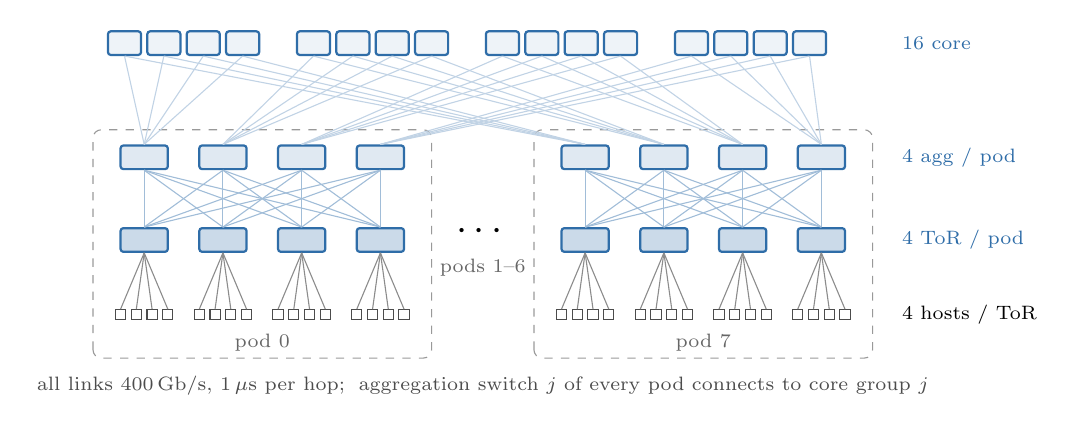
\begin{tikzpicture}[x=1cm,y=1cm,font=\scriptsize,
  core/.style={draw=fabric,fill=fabric!8,thick,rounded corners=1pt,minimum width=0.42cm,minimum height=0.3cm,inner sep=0pt},
  agg/.style={draw=fabric,fill=fabric!15,thick,rounded corners=1pt,minimum width=0.6cm,minimum height=0.3cm,inner sep=0pt},
  tor/.style={draw=fabric,fill=fabric!25,thick,rounded corners=1pt,minimum width=0.6cm,minimum height=0.3cm,inner sep=0pt},
  host/.style={draw=black!70,fill=white,minimum size=0.13cm,inner sep=0pt}]
  % core: 4 groups of 4
  \foreach \g in {0,...,3}
    \foreach \c in {0,...,3}
      \node[core] (c\g\c) at ({0.25+\g*2.4+\c*0.5},4.0) {};
  \node[anchor=west,text=fabric] at (10.0,4.0) {16 core};
  % two pods drawn: 0 and 7
  \foreach \p/\px in {0/0.0,7/5.6} {
    \draw[black!40,rounded corners=3pt,dashed] (\px-0.15,0.0) rectangle (\px+4.15,2.9);
    \node[text=black!60] at (\px+2.0,0.2) {pod \p};
    \foreach \a in {0,...,3} {
      \node[agg] (a\p\a) at ({\px+0.5+\a*1.0},2.55) {};
      \node[tor] (t\p\a) at ({\px+0.5+\a*1.0},1.5) {};
    }
    \foreach \a in {0,...,3}
      \foreach \b in {0,...,3}
        \draw[fabric!45] (t\p\a.north) -- (a\p\b.south);
    \foreach \a in {0,...,3}
      \foreach \h in {0,...,3} {
        \node[host] (h\p\a\h) at ({\px+0.5+\a*1.0+(\h-1.5)*0.2},0.55) {};
        \draw[black!45] (h\p\a\h.north) -- (t\p\a.south);
      }
    % agg a -> core group a
    \foreach \a in {0,...,3}
      \foreach \c in {0,...,3}
        \draw[fabric!30] (a\p\a.north) -- (c\a\c.south);
  }
  \node at (4.8,1.6) {\Large $\cdots$};
  \node[text=black!60] at (4.8,1.15) {pods 1--6};
  \node[anchor=west,text=fabric] at (10.0,2.55) {4 agg / pod};
  \node[anchor=west,text=fabric] at (10.0,1.5) {4 ToR / pod};
  \node[anchor=west] at (10.0,0.55) {4 hosts / ToR};
  \node[align=center,text=black!70] at (4.8,-0.35)
    {all links 400\,Gb/s, 1\,$\mu$s per hop;\; aggregation switch $j$ of every pod connects to core group $j$};
\end{tikzpicture}}
\caption{The 128-node, three-tier full-bisection fat-tree (two of eight pods
drawn). Each ToR has as many uplinks as hosts, and any two pods are joined by
16 paths. The 1024-node tree has the same structure with 16 pods of 64 hosts,
8 switches per tier per pod, 64 core switches and 64 inter-pod paths.}
\label{fig:fattree}
\end{figure}

% load-balancing illustration removed (not needed)
\iffalse
\begin{figure*}[t]
\centering
\resizebox{0.95\textwidth}{!}{%
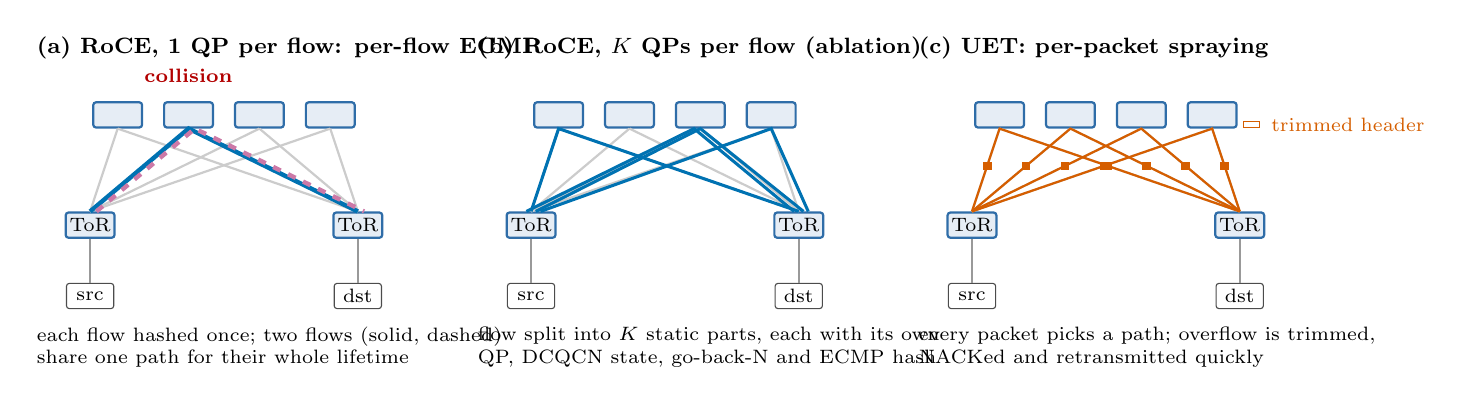
\begin{tikzpicture}[x=1cm,y=1cm,font=\scriptsize,
  sw/.style={draw=fabric,fill=fabric!12,thick,rounded corners=1pt,minimum width=0.62cm,minimum height=0.32cm,inner sep=0pt},
  ep/.style={draw=black!70,fill=white,rounded corners=1pt,minimum width=0.6cm,minimum height=0.32cm,inner sep=0pt},
  pkt/.style={minimum width=0.11cm,minimum height=0.11cm,inner sep=0pt}]
  \foreach \P/\ox/\ttl in {0/0/{(a) RoCE, 1 QP per flow: per-flow ECMP},
                           1/5.6/{(b) RoCE, $K$ QPs per flow (ablation)},
                           2/11.2/{(c) UET: per-packet spraying}} {
    \begin{scope}[xshift=\ox cm]
      \node[font=\footnotesize\bfseries,anchor=west] at (-0.2,3.35) {\ttl};
      \node[ep] (s\P) at (0.6,0.2) {src};
      \node[ep] (d\P) at (4.0,0.2) {dst};
      \node[sw] (L\P) at (0.6,1.1) {ToR};
      \node[sw] (R\P) at (4.0,1.1) {ToR};
      \foreach \k in {0,...,3}
        \node[sw] (u\P\k) at ({0.95+\k*0.9},2.5) {};
      \foreach \k in {0,...,3} {
        \draw[black!20,thick] (L\P.north) -- (u\P\k.south);
        \draw[black!20,thick] (u\P\k.south) -- (R\P.north);
      }
      \draw[black!40,thick] (s\P) -- (L\P); \draw[black!40,thick] (d\P) -- (R\P);
    \end{scope}
  }
  % (a) two flows hash to the same uplink
  \draw[flowA,line width=1.6pt] (L0.north) -- (u01.south) -- (R0.north);
  \draw[flowB,line width=1.6pt,dashed] ($(L0.north)+(0.08,0)$) -- ($(u01.south)+(0.08,0)$) -- ($(R0.north)+(0.08,0)$);
  \node[text=red!70!black,font=\scriptsize\bfseries] at (1.85,3.0) {collision};
  \node[align=left,anchor=west] at (-0.2,-0.45) {each flow hashed once; two flows (solid, dashed)\\share one path for their whole lifetime};
  % (b) K=4 subflows, each hashed independently
  \begin{scope}[xshift=5.6cm]
  \end{scope}
  \draw[flowA,line width=1.1pt] (L1.north) -- (u10.south) -- (R1.north);
  \draw[flowA,line width=1.1pt] ($(L1.north)+(0.06,0)$) -- ($(u12.south)+(0.0,0)$) -- ($(R1.north)+(0.06,0)$);
  \draw[flowA,line width=1.1pt] ($(L1.north)+(-0.06,0)$) -- ($(u12.south)+(-0.08,0)$) -- ($(R1.north)+(-0.06,0)$);
  \draw[flowA,line width=1.1pt] ($(L1.north)+(0.12,0)$) -- (u13.south) -- ($(R1.north)+(0.12,0)$);
  \node[align=left,anchor=west] at (5.4,-0.45) {flow split into $K$ static parts, each with its own\\QP, DCQCN state, go-back-N and ECMP hash};
  % (c) spray: packets on every path
  \foreach \k in {0,...,3} {
    \draw[uet,line width=0.8pt] (L2.north) -- (u2\k.south) -- (R2.north);
    \node[pkt,fill=uet] at ($(L2.north)!0.55!(u2\k.south)$) {};
    \node[pkt,fill=uet] at ($(u2\k.south)!0.45!(R2.north)$) {};
  }
  \node[pkt,draw=uet,fill=white,minimum width=0.2cm,minimum height=0.07cm] (trim) at ($(u23.south)+(0.5,0.05)$) {};
  \node[anchor=west,text=uet] at ($(trim.east)+(0.02,0)$) {trimmed header};
  \node[align=left,anchor=west] at (11.0,-0.45) {every packet picks a path; overflow is trimmed,\\NACKed and retransmitted quickly};
\end{tikzpicture}}
\caption{How each arm uses the paths of the fat-tree. (a) RoCE/DCQCN as
deployed: one QP per flow, one ECMP path per QP. (b) The RoCE multipath arm:
each flow is split into $K$ equal parts on $K$ independent QPs; parts may
still collide. (c) UET: per-packet spraying over all paths. The UET
single-path arm of the ablation behaves like (a), with UET's transport.}
\label{fig:lb}
\end{figure*}
\fi

The rail-optimized GPU cluster with NVLink is described with its results in
Section~\ref{sec:rail}.

\subsection{Workloads}
Table~\ref{tab:workloads} and Fig.~\ref{fig:workloads} summarize the traffic.
Flat-fabric patterns use flow sizes of 16, 64 and 100\,MB. All-to-all and ring
all-reduce were run at 128 nodes only, because the 1024-node versions exceeded
our memory budget; UET ring all-reduce at 64 and 100\,MB did too. Ring
all-reduce and the rail-aware collectives are \emph{trigger-chained}: a flow
starts when its predecessor on the same GPU finishes, so flow completion time
(FCT) includes waiting time and only the makespan is comparable across them.
The rail-aware collectives keep every flow either inside a server (NVLink) or
inside one rail, so they never need to cross rails.

\begin{table}[t]
\centering
\caption{Workloads. $N$ = number of nodes, $S$ = flow size.}
\label{tab:workloads}
\footnotesize
\setlength{\tabcolsep}{3pt}
\begin{tabular}{@{}>{\raggedright\arraybackslash}p{0.17\columnwidth}>{\raggedright\arraybackslash}p{0.22\columnwidth}>{\raggedright\arraybackslash}p{0.55\columnwidth}@{}}
\toprule
\textbf{Short} & \textbf{Pattern} & \textbf{Definition (what it mimics)} \\
\midrule
\wl{PermRand} & Permutation (random) & $N$ flows, random permutation (shuffle) \\
\wl{PermBis}  & Permutation (bisection) & node $i \to i{+}N/2$; every flow crosses the bisection \\
\wl{IncRand}  & Incast (random) & $N{-}1$ senders $\to$ node 0 (storage read, gather) \\
\wl{IncRem}   & Incast (remote) & far half of the fabric ($N/2$ senders) $\to$ node 0 \\
\wl{OutInc}   & Outcast-incast & $N/8$ senders $\to$ node 0; each also sends to 3 others \\
\wl{A2A}      & All-to-all & all $N(N{-}1)$ pairs at once, $S$ per pair \\
\wl{RingAR}   & Ring all-reduce & trigger-chained ring, $2(N{-}1)$ steps per node \\
\midrule
\multicolumn{2}{@{}l}{Rail all-reduce} & NVLink reduce-scatter, rail-local recursive halving/doubling, NVLink all-gather \\
\multicolumn{2}{@{}l}{Rail MoE all-to-all} & NVLink shuffle to the destination rail, then rail-local all-to-all ($S$ per GPU in total) \\
\bottomrule
\end{tabular}
\end{table}

\begin{figure*}[t]
\centering
\resizebox{\textwidth}{!}{%
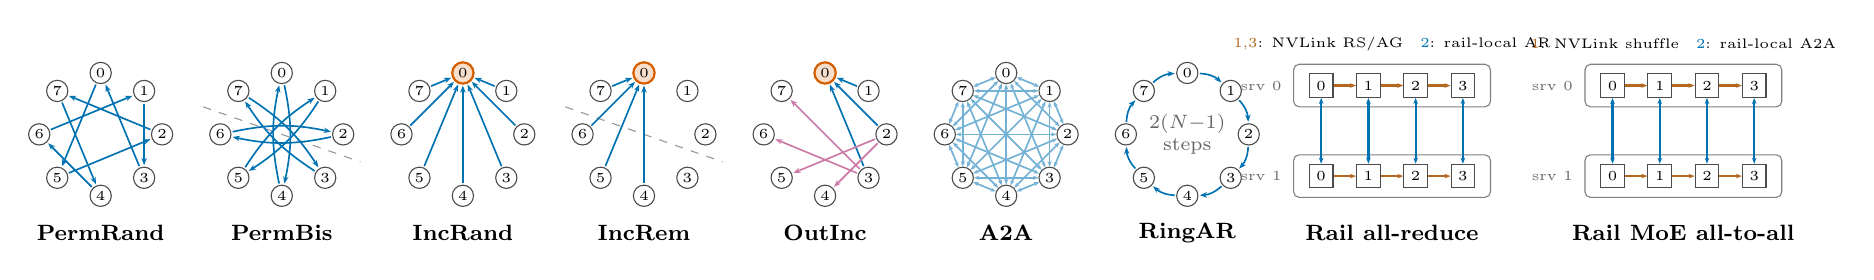
\begin{tikzpicture}[x=1cm,y=1cm,font=\scriptsize,
  nd/.style={circle,draw=black!70,fill=white,minimum size=0.27cm,inner sep=0pt,font=\tiny},
  hot/.style={circle,draw=uet,fill=uet!20,thick,minimum size=0.27cm,inner sep=0pt,font=\tiny},
  fl/.style={-{Stealth[length=2.6pt]},roce,semithick,shorten >=0.5pt,shorten <=0.5pt},
  fl2/.style={-{Stealth[length=2.6pt]},flowB,semithick,shorten >=0.5pt,shorten <=0.5pt},
  gpu/.style={draw=black!70,fill=white,minimum size=0.3cm,inner sep=0pt,font=\tiny}]
  % 1 PermRand
  \begin{scope}[xshift=0cm]
    \ring{a}
    \foreach \s/\d in {0/5,1/3,2/7,3/0,4/6,5/2,6/1,7/4} \draw[fl] (a\s) -- (a\d);
    \node[font=\footnotesize\bfseries] at (0,-1.25) {PermRand};
  \end{scope}
  % 2 PermBis
  \begin{scope}[xshift=2.3cm]
    \ring{b}
    \draw[black!40,dashed] (-1.0,0.35) -- (1.0,-0.35);
    \foreach \s in {0,...,3} {\pgfmathtruncatemacro{\d}{\s+4}\draw[fl] (b\s) to[bend left=12] (b\d);
                               \draw[fl] (b\d) to[bend left=12] (b\s);}
    \node[font=\footnotesize\bfseries] at (0,-1.25) {PermBis};
  \end{scope}
  % 3 IncRand
  \begin{scope}[xshift=4.6cm]
    \ring{c} \node[hot] at (c0) {0};
    \foreach \s in {1,...,7} \draw[fl] (c\s) -- (c0);
    \node[font=\footnotesize\bfseries] at (0,-1.25) {IncRand};
  \end{scope}
  % 4 IncRem
  \begin{scope}[xshift=6.9cm]
    \ring{e} \node[hot] at (e0) {0};
    \draw[black!40,dashed] (-1.0,0.35) -- (1.0,-0.35);
    \foreach \s in {4,...,7} \draw[fl] (e\s) -- (e0);
    \node[font=\footnotesize\bfseries] at (0,-1.25) {IncRem};
  \end{scope}
  % 5 OutInc
  \begin{scope}[xshift=9.2cm]
    \ring{f} \node[hot] at (f0) {0};
    \foreach \s in {1,2,3} \draw[fl] (f\s) -- (f0);
    \draw[fl2] (f2) -- (f4); \draw[fl2] (f2) -- (f5);
    \draw[fl2] (f3) -- (f6); \draw[fl2] (f3) -- (f7);
    \node[font=\footnotesize\bfseries] at (0,-1.25) {OutInc};
  \end{scope}
  % 6 A2A
  \begin{scope}[xshift=11.5cm]
    \ring{g}
    \foreach \s in {0,...,7} {\foreach \d in {0,...,7} {%
      \ifnum\s<\d \draw[roce!55,semithick,{Stealth[length=2pt]}-{Stealth[length=2pt]}] (g\s) -- (g\d); \fi}}
    \node[font=\footnotesize\bfseries] at (0,-1.25) {A2A};
  \end{scope}
  % 7 RingAR
  \begin{scope}[xshift=13.8cm]
    \ring{h}
    \foreach \s in {0,...,7} {\pgfmathtruncatemacro{\d}{mod(\s+1,8)}\draw[fl] (h\s) to[bend left=20] (h\d);}
    \node[font=\scriptsize,align=center,text=black!60] at (0,0) {$2(N{-}1)$\\steps};
    \node[font=\footnotesize\bfseries] at (0,-1.25) {RingAR};
  \end{scope}
  % 8/9 rail-aware collectives: 2 servers x 4 GPUs
  \foreach \P/\ox/\name/\ph in {0/16.4/{Rail all-reduce}/{\textcolor{nvl}{1,3}: NVLink RS/AG\;\; \textcolor{roce}{2}: rail-local AR},
                                1/20.1/{Rail MoE all-to-all}/{\textcolor{nvl}{1}: NVLink shuffle\;\; \textcolor{roce}{2}: rail-local A2A}} {
    \begin{scope}[xshift=\ox cm]
      \foreach \s in {0,1} {
        \draw[black!50,rounded corners=2pt] (-1.25,{0.62-\s*1.15-0.27}) rectangle (1.25,{0.62-\s*1.15+0.27});
        \node[anchor=east,text=black!60,font=\tiny] at (-1.28,{0.62-\s*1.15}) {srv \s};
        \foreach \k in {0,...,3} \node[gpu] (r\P\s\k) at ({-0.9+\k*0.6},{0.62-\s*1.15}) {\k};
      }
      \foreach \s in {0,1} \foreach \k in {0,1,2} {\pgfmathtruncatemacro{\n}{\k+1}
        \draw[-{Stealth[length=2.2pt]},nvl,thick] (r\P\s\k) -- (r\P\s\n);}
      \foreach \k in {0,...,3} \draw[{Stealth[length=2.2pt]}-{Stealth[length=2.2pt]},roce,thick] (r\P0\k) -- (r\P1\k);
      \node[font=\footnotesize\bfseries] at (0,-1.25) {\name};
      \node[font=\tiny,align=center] at (0,1.15) {\ph};
    \end{scope}
  }
\end{tikzpicture}}
\caption{The traffic patterns, drawn for eight nodes (the real runs use 128 or
1024 nodes, and 1024 or 2048 GPUs for the rail-aware collectives). The orange
node is the incast receiver. In OutInc the incast senders also fan out to
other nodes (pink). In the rail-aware collectives, orange arrows are NVLink
phases inside a server and blue arrows are rail-local phases between GPUs on
the same rail; no flow crosses rails.}
\label{fig:workloads}
\end{figure*}

\subsection{Metrics and statistics}
\emph{Makespan} (time until the last flow completes) is the headline metric. We
also record per-tier link utilization and each stack's native congestion cost:
the trim rate NACKs/(new\,+\,retransmitted) for UET, and PFC pause count, pause
time and peak buffer occupancy for RoCE/DCQCN. A lossless run that ever exceeds
its buffer would be flagged as misconfigured; none did.

htsim is deterministic for a fixed seed. The seed sets each switch's ECMP hash
salt and path permutation, so each seed is an equally valid draw of where flows
land. Every configuration is the mean of five seeds: 350 runs on the flat
fat-trees, 240 runs in the multipath ablation and 240 runs on the GPU
cluster, 830 simulations in total. Stack and arm comparisons use Welch's $t$-test at
$p{<}0.05$, and error bars are $t$-based 95\% confidence intervals.

% -----------------------------------------------------------------------------
\section{Results on the Flat Fat-Tree}

\subsection{Speed on the flat fat-tree}
\label{sec:flat}

\begin{figure}[t]
\centering
\includegraphics[width=0.95\columnwidth]{fig_flat_ratio.png}
\caption{RoCE/DCQCN makespan divided by UET makespan on the full-bisection
fat-tree (mean of 5 seeds; row label = pattern $\cdot$ nodes). Values above 1
mean UET is faster. All 34 differences are significant (Welch $p{<}0.05$).
--- = not run (memory budget).}
\label{fig:ratio}
\end{figure}

% absolute-makespan figure removed to keep the page count down (kept for easy revert)
\iffalse
\begin{figure*}[t]
\centering
\includegraphics[width=0.85\textwidth]{fig_flat_makespan.png}
\caption{Absolute makespan at 16\,MB, the size at which every pattern exists on
both stacks (log scale; mean $\pm$ 95\% CI over 5 seeds).}
\label{fig:makespan}
\end{figure*}
\fi

Fig.~\ref{fig:ratio} shows the ratio of RoCE/DCQCN to UET makespan for every
fat-tree configuration.
All 34 differences are statistically significant. UET is faster in 28.

\textbf{Permutation: the load-balancing gap.}
The largest gap is on permutation traffic: a median of 6.4$\times$, with a
range of 5.1--8.5$\times$, and larger at 1024 nodes than at 128. UET comes
close to the line-rate bound. A 16\,MB permutation completes in
388--421\,$\mu$s against an ideal of 320\,$\mu$s, while RoCE/DCQCN needs
2.2--3.4\,ms. Spraying spreads every flow over all paths. Per-flow ECMP instead
lets several flows hash onto one link, and those flows then share it for their
whole lifetime, although the fabric has enough capacity for all of them.
Larger flows shrink the gap slightly (6.65$\times$ at 16\,MB to 5.38$\times$ at
100\,MB for random permutation at 128 nodes), likely because DCQCN's
start-up and recovery transients weigh less in longer flows.

\textbf{Incast and collectives.}
On incast and outcast-incast at 128 nodes UET is 1.3--1.6$\times$ faster.
It drains the 127-to-1 incast in 41.4\,ms, within 2\% of the 40.6\,ms that
the receiver's 400\,Gb/s port allows, while RoCE/DCQCN needs 55.4\,ms.
All-to-all is 1.52$\times$ faster at every size and ring all-reduce
3.40$\times$.

\textbf{Where RoCE/DCQCN wins.}
All six RoCE/DCQCN wins are incast at 1024 nodes: 7\% on random incast and
0.5\% on remote incast, at all three sizes. There, up to 1023 senders converge
on one port, so spraying has nothing to spread. UET then pays for its
loss-based design: 84\% of its random-incast transmissions are trimmed, and
most packets are sent more than once. PFC instead holds senders back without
retransmitting.

\subsection{What each stack pays}
\label{sec:cost}

\begin{figure}[t]
\centering
\includegraphics[width=\columnwidth]{fig_cost.png}
\caption{The two currencies of congestion. Left: UET trim rate (\% of all
transmissions). Right: RoCE/DCQCN cumulative PFC pause time summed over all
ports (log scale). Mean $\pm$ 95\% CI over 5 seeds; row = pattern $\cdot$ nodes.}
\label{fig:cost}
\end{figure}

\begin{figure}[t]
\centering
\includegraphics[width=0.9\columnwidth]{fig_util.png}
\caption{Mean link utilization per tier and direction, 128 nodes, 16\,MB flows
(mean of 5 seeds).}
\label{fig:util}
\end{figure}

The stacks pay for congestion in different currencies (Fig.~\ref{fig:cost}).

\textbf{UET spends bandwidth.}
Its trim rate is at most 3.2\% on permutation, outcast-incast, all-to-all and
ring all-reduce. Incast is the exception: 7--11\% on random and 1--6\% on
remote incast at 128 nodes, and 60\% (remote) and 84\% (random) at 1024 nodes,
independent of flow size. In exchange, spraying keeps the fabric busy (Fig.~\ref{fig:util}):
0.73--0.85 mean utilization on every tier for permutation, and up to 0.99 for
all-to-all.

\textbf{RoCE/DCQCN spends time.}
It never drops a packet and never exceeded its lossless buffer; peak occupancy
stays at 0.16--0.17\,MB on every workload. The price is back-pressure. PFC
pause is negligible on permutation ($\le$0.07 port-seconds) but reaches
2--13 port-seconds on all-to-all, and 540--3{,}350 port-seconds on 1024-node
random incast. Single-path hashing and DCQCN pacing also leave capacity unused:
on permutation every tier runs at only 0.13--0.17 utilization, about a fifth of
UET's, and on all-to-all and ring all-reduce at 0.57--0.65 and 0.17--0.19
against UET's 0.87--0.99 and 0.57--0.64. On incast both stacks leave the fabric
almost idle (0.01): the receiver's port is the only bottleneck.


\begin{figure}[t]
\centering
\resizebox{\columnwidth}{!}{%
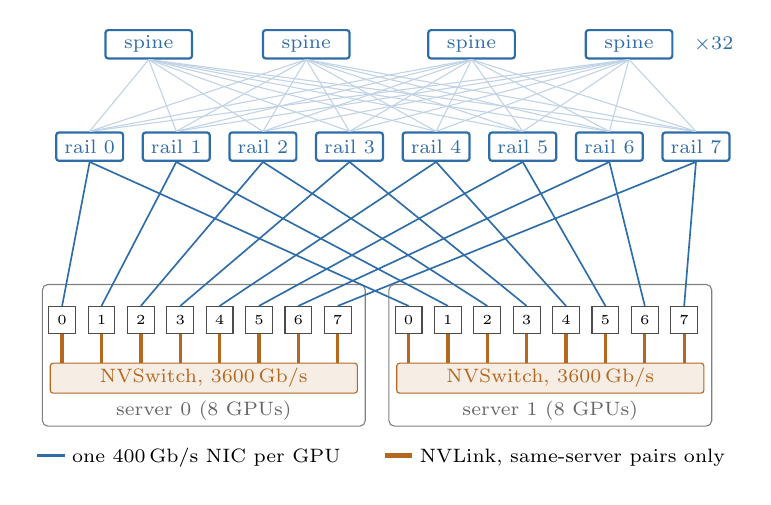
\begin{tikzpicture}[x=1cm,y=1cm,font=\scriptsize,
  sw/.style={draw=fabric,thick,rounded corners=1pt,minimum height=0.36cm,inner sep=1pt,text=fabric},
  gpu/.style={draw=black!70,fill=white,minimum size=0.34cm,inner sep=0pt,font=\tiny}]
  \foreach \i/\x in {0/1.2,1/3.2,2/5.3,3/7.3}
    \node[sw,minimum width=1.1cm] (sp\i) at (\x,4.0) {spine};
  \node[anchor=west,text=fabric] at (8.0,4.0) {$\times$32};
  \foreach \k in {0,...,7}
    \node[sw,minimum width=0.85cm] (L\k) at ({0.45+\k*1.1},2.7) {rail \k};
  \foreach \k in {0,...,7}
    \foreach \i in {0,...,3}
      \draw[fabric!30] (L\k.north) -- (sp\i.south);
  \foreach \s in {0,1} {
    \draw[black!50,rounded corners=2pt] ({\s*4.4-0.15},-0.85) rectangle ({\s*4.4+3.95},0.95);
    \node[anchor=south,inner sep=2pt,text=black!60] at ({\s*4.4+1.9},-0.85) {server \s{} (8 GPUs)};
    \foreach \k in {0,...,7} {
      \node[gpu] (g\s\k) at ({\s*4.4+0.1+\k*0.5},0.5) {\k};
      \draw[fabric,semithick] (g\s\k.north) -- (L\k.south);
      \draw[nvl,very thick] (g\s\k.south) -- ++(0,-0.38);
    }
    \draw[nvl,fill=nvl!12,rounded corners=1pt] ({\s*4.4-0.05},-0.43) rectangle ({\s*4.4+3.85},-0.05);
    \node[text=nvl] at ({\s*4.4+1.9},-0.24) {NVSwitch, 3600\,Gb/s};
  }
  % ---- (b) flat-control panel removed (not needed); kept for easy revert ----
\iffalse
  % ---- (b) flat control ----
  \begin{scope}[yshift=-6.4cm]
  \node[font=\footnotesize\bfseries,anchor=west] at (-0.2,4.55) {(b) flat control (same switches)};
  \foreach \i/\x in {0/1.2,1/3.2,2/5.3,3/7.3}
    \node[sw,minimum width=1.1cm] (fsp\i) at (\x,4.0) {spine};
  \node[anchor=west,text=fabric] at (8.0,4.0) {$\times$32};
  \node[sw,minimum width=2.6cm] (FL0) at (1.9,2.7) {leaf 0: servers 0--3};
  \node[sw,minimum width=2.6cm] (FL1) at (6.3,2.7) {leaf 1: servers 4--7};
  \foreach \l in {0,1}
    \foreach \i in {0,...,3}
      \draw[fabric!30] (FL\l.north) -- (fsp\i.south);
  \foreach \s in {0,1} {
    \draw[black!50,rounded corners=2pt] ({\s*4.4-0.15},-0.85) rectangle ({\s*4.4+3.95},0.95);
    \node[anchor=south,inner sep=2pt,text=black!60] at ({\s*4.4+1.9},-0.85) {server \ifnum\s=0 0\else 4\fi{} (8 GPUs)};
    \foreach \k in {0,...,7} {
      \node[gpu] (fg\s\k) at ({\s*4.4+0.1+\k*0.5},0.5) {\k};
      \draw[fabric,semithick] (fg\s\k.north) -- (FL\s.south);
      \draw[nvl,very thick] (fg\s\k.south) -- ++(0,-0.38);
    }
    \draw[nvl,fill=nvl!12,rounded corners=1pt] ({\s*4.4-0.05},-0.43) rectangle ({\s*4.4+3.85},-0.05);
    \node[text=nvl] at ({\s*4.4+1.9},-0.24) {NVSwitch, 3600\,Gb/s};
  }
  \end{scope}
\fi
  \node[align=center] at (4.15,-1.25)
    {\textcolor{fabric}{\rule[2pt]{10pt}{1pt}}~one 400\,Gb/s NIC per GPU\qquad
     \textcolor{nvl}{\rule[1.5pt]{10pt}{2pt}}~NVLink, same-server pairs only};
\end{tikzpicture}}
\caption{The two-plane GPU cluster (two of 128/256 servers shown). Every GPU
has two egress planes: a flow between GPUs of the same server uses the
server's NVLink switch, any other flow uses the 400\,Gb/s fabric, where GPU
$k$ of every server attaches to a leaf of rail~$k$ (one leaf per rail drawn;
4 or 8 in the real cluster).}
\label{fig:railtopo}
\end{figure}

% rail figures defined before the section heading (figure* lands >= 1 page after definition)
\begin{figure*}[t]
\centering
\includegraphics[width=\textwidth]{fig_rail_vs_flat.png}
\caption{Makespan on the 1024- and 2048-GPU clusters with NVLink: rail
placement (solid) next to flat placement (hatched), for both stacks. Left:
rail-aware all-reduce. Right: rail-aware MoE all-to-all. Mean $\pm$ 95\% CI
over 5 seeds.}
\label{fig:railms}
\end{figure*}

\begin{figure*}[t]
\centering
\includegraphics[width=\textwidth]{fig_rail_benefit.png}
\caption{Makespan change from rail placement relative to flat placement
(negative = rails faster). Filled markers are significant (Welch $p{<}0.05$);
faint dots are individual seeds.}
\label{fig:rail}
\end{figure*}

% =============================================================================
\section{Rail-Optimized GPU Clusters with NVLink}
\label{sec:rail}

\begin{figure*}[t]
\centering
\includegraphics[width=\textwidth]{fig_rail_cost_flat.png}
\caption{Congestion cost of rail-aware MoE all-to-all, rail placement (solid,
value labelled) next to flat placement (hatched). Left: RoCE/DCQCN cumulative
PFC pause time. Right: UET retransmitted packets. Mean $\pm$ 95\% CI over 5
seeds.}
\label{fig:railcost}
\end{figure*}

The fat-tree of Section~\ref{sec:flat} treats every GPU as an independent
endpoint. Production AI clusters are built differently: GPUs sit eight to a
server behind an NVLink switch, and each GPU has its own NIC wired to a
different leaf switch, its \emph{rail}. Collectives are written for this
structure, so that traffic stays either inside a server or inside a rail. We
model such clusters to see how the two transports behave on them and how much
rail placement is worth to each.

\subsection{Cluster and NVLink model}

We model 1024 and 2048 GPUs as DGX H100-like servers of 8 GPUs, each GPU with
its own 400\,Gb/s NIC on its own rail, in a two-tier non-blocking leaf-spine
with 64-port leaves (32 down, 32 up) and 32 spines. A leaf holds one GPU from
each of 32 servers, so traffic between GPUs of the same rail index stays on
that rail's leaves and the spines above them. NVLink4 is modelled as a second
topology: one 3600\,Gb/s crossbar per server with 100\,ns links. Each flow is
routed at connection time over NVLink if both endpoints share a server, and
over the rail fabric otherwise. The simulator checks that each plane's link
capacity matches its host injection rate, because a mismatch silently
throttles traffic to the slower of the two. Fig.~\ref{fig:railtopo} sketches
the cluster. To measure what rail placement itself is worth, every
configuration is also run with a \emph{flat} placement: the same switches and
links, but each leaf serves four whole servers. NVLink is enabled in both, so
only the host-to-leaf assignment differs.


\subsection{Rail-aware collectives}

We run the two collectives that rail-optimized clusters are built for
(Table~\ref{tab:workloads}, Fig.~\ref{fig:workloads}). The \emph{rail-aware
all-reduce} is the hierarchical algorithm used on DGX systems: an intra-server
reduce-scatter over NVLink, a rail-local all-reduce by recursive halving and
doubling, and an intra-server all-gather over NVLink. The \emph{rail-aware MoE
all-to-all} is the Mixture-of-Experts dispatch pattern: an NVLink shuffle
places the data for rail $r$ on the server's GPU at rail $r$, followed by a
rail-local all-to-all. No flow in either collective crosses rails. Each runs
at 16, 64 and 100\,MB (for MoE, the total volume each GPU dispatches) on both
cluster sizes, both placements and both stacks, with five seeds each (240 runs).



\subsection{Rails help both transports}

Fig.~\ref{fig:railms} shows the makespans and Fig.~\ref{fig:rail} the change
that rail placement brings. RoCE/DCQCN gains 8--41\%, significant in all 12
configurations. The largest gains are on MoE all-to-all: $-41\%$ at 1024
GPUs/16\,MB and $-33\%$ at 2048 GPUs/64\,MB. UET gains 3--10\%, significant in
10 of 12; the two exceptions are within $\pm$4\%. Spraying already avoids hot
paths, so UET has less to gain, but rails are not only an optimization for
per-flow ECMP.

\subsection{RoCE/DCQCN versus UET on the cluster}

\begin{figure}[t]
\centering
\includegraphics[width=0.95\columnwidth]{fig_rail_ratio.png}
\caption{RoCE/DCQCN makespan divided by UET makespan on the GPU cluster, rail
placement (filled) and flat placement (hollow); AR = rail-aware all-reduce,
MoE = rail-aware MoE all-to-all, then GPUs and size. Values above 1 mean UET
is faster. Mean $\pm$ propagated 95\% CI over 5 seeds.}
\label{fig:railratio}
\end{figure}

Fig.~\ref{fig:railratio} compares the two stacks under both placements.

\textbf{All-reduce: UET far ahead, without congestion.}
UET finishes the rail-aware all-reduce 1.7$\times$ faster at 16\,MB and
4.2--4.6$\times$ faster at 64--100\,MB on rails (1.7--5.4$\times$ with flat
placement). Neither stack is congested on this collective: RoCE/DCQCN
accumulates at most 0.11 port-seconds of PFC pause, and UET retransmits fewer
than 0.02\,M packets. The difference is how much of the fabric each stack
uses: under RoCE/DCQCN the fabric links run at 0.07--0.18 mean utilization,
under UET at 0.26--0.44.

\textbf{MoE all-to-all: rails nearly close the gap.}
With flat placement UET is 1.21--1.86$\times$ faster on MoE all-to-all. Rails
bring RoCE/DCQCN to within 1.02--1.33$\times$, and at 1024 GPUs/64\,MB the two
are statistically tied (1.02$\times$, $p{=}0.18$).


\subsection{What rails save, and how cost scales}

\textbf{Mechanism.}
MoE all-to-all is the collective on which both stacks pay for congestion
(Fig.~\ref{fig:railcost}). For RoCE/DCQCN, rails relieve back-pressure: PFC
pause time falls 26--59\% in every MoE configuration. For UET the effect is
mixed. Rails cut retransmissions by 11--19\% in three of the 64--100\,MB
configurations but leave them within $\pm$5\% in the others. This suggests
that part of UET's MoE loss is generated at the receiving endpoint, which no
change of topology relieves.

\textbf{Congestion cost grows faster than the cluster.}
On rails, doubling from 1024 to 2048 GPUs (MoE, 100\,MB) multiplies
RoCE/DCQCN pause time by 4.7$\times$ (7.2$\to$33.7 port-s) and UET
retransmissions by 3.3$\times$ (7.5\,M$\to$25\,M). At 64\,MB the two diverge:
RoCE/DCQCN pause time triples (6.1$\to$19.0 port-s), while UET's
retransmissions stay flat (6.8\,M$\to$6.6\,M).

% ---- rail-only version of this section (previous draft), kept for easy revert ----
\iffalse
\subsection{Rail-optimized clusters with NVLink}


\begin{figure}[t]
\centering
\includegraphics[width=0.78\columnwidth]{fig_rail_makespan.png}
\caption{Makespan on the rail-optimized 1024- and 2048-GPU clusters with
NVLink (mean $\pm$ 95\% CI over 5 seeds). Labels give RoCE/DCQCN makespan
divided by UET makespan; bold = significant (Welch $p{<}0.05$), n.s.\ = not.}

\end{figure}

Fig.~\ref{fig:railms} compares the two stacks on the cluster of
Fig.~\ref{fig:railtopo}. The intra-server phases of both collectives run on
NVLink, so the 400\,Gb/s fabric carries only rail-local traffic.

\textbf{All-reduce: UET far ahead, without congestion.}
UET finishes the rail-aware all-reduce 1.7$\times$ faster at 16\,MB and
4.2--4.6$\times$ faster at 64--100\,MB, at both cluster sizes. Neither stack is
congested on this collective: RoCE/DCQCN accumulates at most 0.11
port-seconds of PFC pause, and UET retransmits fewer than 0.02\,M packets. The
difference is how much of the fabric each stack uses: under RoCE/DCQCN the
fabric links run at 0.07--0.18 mean utilization, under UET at 0.26--0.44.

\begin{figure}[t]
\centering
\includegraphics[width=0.9\columnwidth]{fig_rail_cost.png}
\caption{Congestion cost of rail-aware MoE all-to-all on the rail-optimized
cluster. Left: RoCE/DCQCN PFC pause time. Right: UET retransmitted packets.
Mean $\pm$ 95\% CI over 5 seeds.}

\end{figure}

\textbf{MoE all-to-all: nearly tied.}
On MoE all-to-all RoCE/DCQCN comes within 1.02--1.33$\times$ of UET; at 1024
GPUs/64\,MB the two are statistically tied (1.02$\times$, $p{=}0.18$). This is
the collective on which both stacks pay for congestion
(Fig.~\ref{fig:railcost}): RoCE/DCQCN accumulates 0.9--33.7 port-seconds of
PFC pause, and UET trims 6--21\% of its transmissions.

\textbf{Congestion cost grows faster than the cluster.}
Doubling from 1024 to 2048 GPUs (MoE, 100\,MB) multiplies RoCE/DCQCN pause
time by 4.7$\times$ (7.2$\to$33.7 port-s) and UET retransmissions by
3.3$\times$ (7.5\,M$\to$25\,M). At 64\,MB the two diverge: RoCE/DCQCN pause
time triples (6.1$\to$19.0 port-s), while UET's retransmissions stay flat
(6.8\,M$\to$6.6\,M).

\fi

% =============================================================================
\section{Multipath Ablation: Spraying versus Transport}
\label{sec:ablation}

\begin{figure*}[t]
\centering
\includegraphics[width=0.95\textwidth]{fig_abl_arms.png}
\caption{Multipath ablation at 16\,MB: makespan of every arm, normalized to
UET with spraying (log scale; mean $\pm$ 95\% CI over 5 seeds). Blue: RoCE/DCQCN
with 1, 2, 4 and 8 QPs per flow. Hatched orange: UET on a single ECMP path.}
\label{fig:abl}
\end{figure*}


The comparisons so far pair each transport with its native load balancer, as
each would be deployed. To separate the two we add two arms
(Table~\ref{tab:stacks}). \emph{UET single-path} keeps
everything about UET except spraying: each flow uses one ECMP path.
\emph{RoCE with $K$ QPs} splits each flow statically into $K$ equal parts on
$K$ independent QPs, each with its own DCQCN state, go-back-N and ECMP hash,
as RDMA libraries do in practice. It gains path diversity without reordering
inside a QP. We run all twelve flat-fabric patterns at 16\,MB with five seeds
per arm (Fig.~\ref{fig:abl}).

\begin{figure}[t]
\centering
\includegraphics[width=\columnwidth]{fig_abl_decomp.png}
\caption{Decomposition of the RoCE/DCQCN-to-UET gap at 16\,MB on a log scale:
transport, measured with both stacks on a single path (RoCE 1 QP vs.\ UET
single-path), and spraying, measured within UET (single-path vs.\ spraying).
The two segments multiply to the total.}
\label{fig:decomp}
\end{figure}

\textbf{Spraying is most of the permutation gap.}
Fig.~\ref{fig:decomp} splits the end-to-end gap into its two factors. On
permutation, spraying alone makes UET 3.5--4.8$\times$ faster, while UET's
transport on a single path beats RoCE/DCQCN by 1.6--1.8$\times$. Spraying is
therefore 69--73\% of the gap on a log scale. It is about half of the gap on
ring all-reduce (1.89$\times$ of 3.40$\times$) and 42\% on all-to-all. On incast
and outcast-incast spraying contributes nothing: single-path and sprayed UET
finish within 0.1\% of each other, because the bottleneck is the receiver's
port, which every path shares.

\textbf{The transport still matters.}
With both stacks on a single path, UET is 1.3--1.8$\times$ faster in ten of the
twelve configurations; only the receiver-bound 1024-node incasts favour
RoCE/DCQCN (0.93--0.99$\times$). On incast and outcast-incast at 128 nodes the
whole 1.3--1.6$\times$ gap is transport. UET reaches line rate at the
receiver, while DCQCN's multiplicative cuts and slow recovery leave the
bottleneck port partly idle even though PFC prevents any loss.

\begin{figure}[t]
\centering
\includegraphics[width=0.92\columnwidth]{fig_abl_kcurve.png}
\caption{RoCE/DCQCN speed-up from splitting each flow over $K$ QPs, relative
to $K{=}1$ (16\,MB; mean $\pm$ 95\% CI over 5 seeds). Solid: 128 nodes;
dashed: 1024 nodes.}
\label{fig:kcurve}
\end{figure}

\textbf{More QPs help RoCE/DCQCN, but do not replace spraying.}
Splitting flows over more QPs speeds RoCE/DCQCN up almost everywhere
(Fig.~\ref{fig:kcurve}). With $K{=}8$ it gains 1.8--2.3$\times$ on permutation,
1.8$\times$ on ring all-reduce, 1.2--1.5$\times$ on 128-node incast and on
outcast-incast, and 1.2--1.3$\times$ on all-to-all, where $K{=}4$ is slightly
better than $K{=}8$. Only the 1024-node incasts, bound by the receiver's port,
do not move ($\le$2\%). On incast the extra QPs cannot add paths at the
bottleneck, so the gain comes from rate control: $K$ independent DCQCN
instances recover from rate cuts in parallel and keep the receiver's port
busier. The cost is more back-pressure: PFC pause time grows 5.9$\times$ on
128-node random incast and 7.9$\times$ on ring all-reduce from $K{=}1$ to $K{=}8$.

With eight QPs RoCE/DCQCN roughly catches up with single-path UET: it is
within 0.88--1.06$\times$ of it in ten of twelve configurations, and identical
on ring all-reduce (1.00$\times$, $p{=}1.0$). It still trails UET with
spraying by 3.2--4.1$\times$ on permutation. Eight static flow parts, each
hashed once, still collide; per-packet spraying spreads load over all 16 or 64
paths and adapts within a flow.

% -----------------------------------------------------------------------------
\section{Discussion and Limitations}
\label{sec:discussion}

\textbf{Load balancing versus transport.}
Our RoCE multipath arm is a static split. RoCE with adaptive routing, or with
packet spraying and an out-of-order receiver, would likely close more of the
permutation gap than extra QPs do.

\textbf{RoCE is not InfiniBand.}
Our lossless baseline is RoCEv2 with PFC and DCQCN. Native InfiniBand uses
credit-based link-level flow control and, in current generations, adaptive
routing. Our results should not be read as an InfiniBand evaluation.

\textbf{Simulation fidelity.}
All results are from htsim. We use 1\,$\mu$s per hop, which is higher than
current switches (roughly 150--450\,ns), so latency-bound phases are pessimistic
for both stacks. DCQCN was run at a single operating point ($K{=}8$) and NSCC at
its defaults. The switch buffers also differ: 1000 packets for RoCE/DCQCN versus
1$\times$BDP for UET, which if anything favours RoCE/DCQCN. Flow sizes are
uniform, and MoE routing is uniform rather than skewed toward hot experts.

\textbf{Coverage gaps.}
UET ring all-reduce at 64 and 100\,MB, and all-to-all and ring all-reduce at
1024 nodes, exceeded our memory budget. The multipath ablation covers 16\,MB
flows only.

% -----------------------------------------------------------------------------
\section{Future Work}
\label{sec:future}

\begin{itemize}
  \item \textbf{Adaptive routing for the lossless baseline}, and the multipath
        ablation on the rail-optimized cluster and at 64--100\,MB.
  \item \textbf{Tuning DCQCN.} Sweeping its ECN threshold and minimum rate
        would show how much of the transport gap is configuration rather than
        design.
  \item \textbf{Other congestion-control algorithms}, beyond DCQCN on the
        lossless side and NSCC on the UET side.
  \item \textbf{Real LLM training traces} (GOAL/ATLAHS) instead of synthetic
        collectives.
\end{itemize}

% -----------------------------------------------------------------------------
\section{Related Work}

DCQCN~\cite{dcqcn} and the operational experience of RoCE at
scale~\cite{rdma-scale} established the lossless-Ethernet design. Its
PFC-related pathologies motivated both better congestion control
(e.g.,~HPCC~\cite{hpcc}) and proposals to drop the lossless requirement
altogether~\cite{irn}. Packet trimming and per-packet spraying were combined in
NDP~\cite{ndp}, which introduced htsim. Spraying's benefits and its reordering
cost were studied in~\cite{spray}, and ECMP flow collisions in~\cite{hedera}.
UET builds on these ideas~\cite{uec-spec,uec-design,reps}. A broader
discussion of datacenter Ethernet for AI and HPC is given
in~\cite{hoefler-ethernet}. Rail-optimized fabrics are standard in GPU
clusters, and~\cite{railonly} argues that much of the spine can be removed for
LLM training. To our knowledge, ours is among the first controlled,
same-simulator comparisons of UET and RoCE/DCQCN that separates multipath from
transport and covers rail-optimized clusters with NVLink.
\todo{check recent UET evaluations (2025--26) and position against them.}

% -----------------------------------------------------------------------------
\section{Conclusion}

In a controlled htsim comparison on full-bisection fabrics, UET is the faster
transport almost everywhere; RoCE/DCQCN wins only when a single receiver port
is the bottleneck at scale. UET pays in bandwidth, RoCE/DCQCN in pause time and
idle capacity. Per-packet spraying explains about 70\% of UET's advantage on
permutation, while on incast all of it is transport. Splitting RoCE flows over eight QPs lets
RoCE/DCQCN match single-path UET, but not sprayed UET. On GPU clusters with
NVLink, rail placement helps both stacks (RoCE/DCQCN by 8--41\%, UET by
3--10\%) and brings RoCE/DCQCN within 1.02--1.33$\times$ of UET on MoE
all-to-all, while UET keeps a 1.7--4.6$\times$ lead on all-reduce.

\section*{Artifact}
Simulator patches (NVLink plane, multi-QP RoCE), traffic matrices, run scripts
and raw results will be released. \todo{repository link.}

% keep every figure ahead of the references; balance the last page's columns
\FloatBarrier
\balance
\bibliographystyle{IEEEtran}
\bibliography{refs}

\end{document}
